% Strip build-host metadata (dates/timezone, trailer ID) from the PDF
\pdfinfoomitdate=1
\pdftrailerid{}
\pdfsuppressptexinfo=-1
\documentclass[10pt,twocolumn,a4paper]{article}

% ------------------------------------------------------------------
% Page layout
% ------------------------------------------------------------------
\usepackage[a4paper,left=0.75in,right=0.75in,top=0.8in,bottom=0.8in,
            columnsep=0.25in]{geometry}
\setlength{\parindent}{1.5em}

% ------------------------------------------------------------------
% Fonts
% ------------------------------------------------------------------
\usepackage[T1]{fontenc}
\usepackage[utf8]{inputenc}
\usepackage{amsmath}
\usepackage{newtxtext,newtxmath}
\usepackage[zerostyle=c,scaled=.94]{newtxtt}
\usepackage{microtype}

% ------------------------------------------------------------------
% Packages
% ------------------------------------------------------------------
\usepackage{cite}
\usepackage{graphicx}
\usepackage{array}
\usepackage{tabularx}
\usepackage{xcolor}
\usepackage{listings}
\usepackage{enumitem}
\usepackage{titlesec}
\usepackage{caption}
\usepackage{tikz}
\usetikzlibrary{positioning,arrows.meta,shapes.geometric,fit,backgrounds,calc}
\usepackage[hidelinks]{hyperref}
\usepackage{url}
\usepackage{orcidlink}
\usepackage{flushend}

\hypersetup{
  pdftitle={Specter OS: A Fail-Closed, Transparently Tor-Routed Live Linux Distribution},
  pdfauthor={Hamza Sajid},
  pdfsubject={Transparent Tor routing and leak prevention in a live Linux distribution},
  pdfkeywords={Tor, anonymity, transparent proxy, iptables, netfilter,
    live operating system, leak prevention, Debian, SquashFS, systemd}
}

% URLs break only after "/", "." or "-"
\def\UrlBreaks{\do\/\do\.\do\-}
\def\UrlBigBreaks{}

% Inline code is never split across two lines
\DeclareRobustCommand{\texttt}[1]{\mbox{\ttfamily #1}}

\setlength{\emergencystretch}{3em}

% ------------------------------------------------------------------
% Headings: "1. Introduction", "2.1. Tor and Transparent Proxying"
% ------------------------------------------------------------------
\renewcommand{\thesection}{\arabic{section}}
\renewcommand{\thesubsection}{\thesection.\arabic{subsection}}
\titleformat{\section}
  {\normalfont\fontsize{12}{14}\selectfont\bfseries\raggedright}
  {\thesection.}{0.5em}{}
\titleformat{\subsection}
  {\normalfont\normalsize\bfseries\raggedright}
  {\thesubsection.}{0.5em}{}
\titlespacing*{\section}{0pt}{12pt}{6pt}
\titlespacing*{\subsection}{0pt}{8pt}{4pt}

% ------------------------------------------------------------------
% Captions: tables above, figures below, 8pt, centred
% ------------------------------------------------------------------
\captionsetup{font=footnotesize, labelsep=period, justification=centering,
              singlelinecheck=false}
\captionsetup[table]{name=TABLE, textfont=sc, position=top, skip=4pt}
\captionsetup[figure]{name=Figure, position=bottom, skip=6pt}
\captionsetup[lstlisting]{position=bottom, skip=4pt}

\setlist{itemsep=1pt, topsep=3pt, parsep=0pt}

% ------------------------------------------------------------------
% Styles
% ------------------------------------------------------------------
\definecolor{boxfill}{RGB}{238,242,248}
\definecolor{torfill}{RGB}{226,238,226}
\definecolor{dropfill}{RGB}{248,228,228}
\definecolor{line}{RGB}{60,60,70}
\definecolor{codebg}{RGB}{247,247,247}

\lstdefinestyle{shell}{
  basicstyle=\fontsize{7.5}{9}\selectfont\ttfamily,
  backgroundcolor=\color{codebg},
  frame=single, framerule=0.3pt, rulecolor=\color{gray!60},
  breaklines=true, breakatwhitespace=true,
  columns=fullflexible, keepspaces=true,
  xleftmargin=3pt, xrightmargin=3pt,
  aboveskip=6pt, belowskip=4pt,
  showstringspaces=false
}

\tikzset{
  >={Stealth[length=2mm]},
  blk/.style={draw=line, fill=boxfill, rounded corners=2pt, align=center,
              font=\footnotesize, text=black, minimum height=6mm, inner sep=3pt},
  tor/.style={blk, fill=torfill},
  drop/.style={blk, fill=dropfill},
  dec/.style={draw=line, fill=white, diamond, aspect=2.2, align=center,
              font=\footnotesize, inner sep=1pt},
  flow/.style={->, draw=line, thick},
}

% Grid table helpers
\newcolumntype{P}[1]{>{\raggedright\arraybackslash}p{#1}}
\newcolumntype{Y}{>{\raggedright\arraybackslash}X}

\setlength{\textfloatsep}{10pt plus 2pt minus 2pt}
\setlength{\floatsep}{8pt plus 2pt minus 2pt}

\begin{document}

% ------------------------------------------------------------------
% Title block
% ------------------------------------------------------------------
\twocolumn[{%
\begin{center}
  {\fontsize{14}{17}\selectfont\bfseries
   Specter OS: A Fail-Closed, Transparently Tor-Routed\\
   Live Linux Distribution\par}
  \vspace{10pt}
  {\fontsize{11}{13}\selectfont
   Hamza Sajid\textsuperscript{1}\,\orcidlink{0009-0007-2231-9783}\par}
  \vspace{5pt}
  {\fontsize{9}{11}\selectfont
   \textsuperscript{1}Department of Computer Science, NUST Balochistan
   Campus (NBC), National University of Sciences and Technology, Pakistan\\
   (e-mail: hamza.bscs23.nbc@student.nust.edu.pk)\par}
\end{center}
\vspace{12pt}
}]
\thispagestyle{plain}
\pagestyle{plain}
\raggedbottom

% ------------------------------------------------------------------
\noindent{\small\bfseries\textit{Abstract}\textemdash
Anonymity tools that rely on per-application proxy configuration fail
silently. One misconfigured program, one IPv6 route or one ICMP probe is
enough to expose the user's real network address. This paper presents
Specter OS, a Debian-based live distribution that runs entirely from
RAM and moves Tor enforcement from user space into the kernel packet
filter. A single \texttt{systemd} unit installs a default-deny
\texttt{netfilter} policy before any network interface is configured.
It redirects TCP to Tor's transparent proxy port and DNS to Tor's
resolver, and it drops everything else, including ICMP and all IPv6
traffic. We describe the threat model, the boot ordering that removes
the early-boot leak window, the firewall rule set, the build pipeline
from \texttt{debootstrap} to a hybrid ISO, and a verification procedure
for each leak vector. We also discuss the limitations of a transparent
proxy design and outline future work toward persistence, UEFI support
and mandatory access control.\par}

\vspace{6pt}
\noindent{\small\bfseries\textit{Index Terms}\textemdash
Tor, anonymity, transparent proxy, iptables, netfilter, live operating
system, leak prevention, Debian, SquashFS, systemd.\par}

% ------------------------------------------------------------------
\section{Introduction}
\label{sec:intro}

Tor~\cite{dingledine2004tor} provides low-latency anonymous
communication by relaying TCP streams through three volunteer-operated
relays. In practice, most deanonymisation of Tor users does not come
from attacks on the Tor protocol. It comes from traffic that never
entered Tor in the first place: DNS queries sent to the local resolver,
UDP-based protocols such as QUIC and WebRTC, ICMP diagnostics, IPv6
connections that bypass an IPv4-only proxy configuration, and packets
sent during the seconds between link-up and the start of the proxy.

Specter OS addresses this class of failure at the operating-system
level. Its design goals are:
\begin{enumerate}
  \item \emph{Transparency:} applications need no proxy settings.
  \item \emph{Fail-closed behaviour:} if Tor is unavailable, the system
        is offline rather than exposed.
  \item \emph{No boot-time window:} enforcement exists before any
        interface obtains an address.
  \item \emph{Amnesia:} the system runs from a read-only compressed
        image in RAM and leaves no state on the host.
  \item \emph{Auditability:} the system is assembled by hand from a
        minimal base, so every component is explicit.
\end{enumerate}

The remainder of this paper is organised as follows.
Section~\ref{sec:background} reviews related systems.
Section~\ref{sec:threat} defines the threat model.
Section~\ref{sec:design} describes the architecture.
Section~\ref{sec:impl} covers the build pipeline.
Section~\ref{sec:eval} presents the verification methodology and results.
Section~\ref{sec:limits} discusses limitations, and
Section~\ref{sec:future} outlines future work.

% ------------------------------------------------------------------
\section{Background and Related Work}
\label{sec:background}

\subsection{Tor and Transparent Proxying}
A Tor client exposes a SOCKS interface for cooperating applications.
For uncooperative applications, Tor offers a \texttt{TransPort}. This
listener accepts connections that the kernel has redirected with
\texttt{netfilter} NAT, and it recovers the original destination with
the \texttt{SO\_ORIGINAL\_DST} socket option~\cite{torproject2024transparent}.
A companion \texttt{DNSPort} resolves names through the Tor network.
\texttt{AutomapHostsOnResolve} maps hostnames, including
\texttt{.onion} names, into a private virtual range so that later TCP
connections can be correlated back to them.

\subsection{Existing Systems}
\textbf{Tails}~\cite{tails} is an amnesic live system that forces
traffic through Tor using a firewall combined with application-level
configuration. \textbf{Whonix}~\cite{whonix} isolates applications in a
workstation virtual machine whose only network path is a separate
gateway VM running Tor, so leaks are prevented by topology rather than
by firewall rules alone. \textbf{Qubes OS}~\cite{qubes} generalises
isolation through hardware virtualisation. Specter OS follows the Tails
model of a single amnesic host. It deliberately keeps the enforcement
mechanism small enough to be read in full, which suits study and
experimentation.

% ------------------------------------------------------------------
\section{Threat Model}
\label{sec:threat}

We consider a \emph{local network observer} (for example an ISP, a Wi-Fi
operator or a captive portal) and a \emph{remote server} that the user
contacts. The adversary's goal is to learn the user's real IP address
or link the user's activity to their identity.

The adversary is assumed to be able to (i) observe all packets on the
local link, (ii) operate a malicious destination server, and (iii)
cause applications to emit non-TCP traffic, for example through
WebRTC~\cite{webrtcleak}.

The following are \emph{out of scope}: global passive adversaries
capable of end-to-end traffic correlation~\cite{murdoch2005low}, browser
fingerprinting, kernel or firmware compromise, and physical access to a
running machine. Table~\ref{tab:vectors} lists the leak vectors that the
design must close.

\begin{table}[t]
\centering
\caption{Leak Vectors and Specter OS Mitigations}
\label{tab:vectors}
\renewcommand{\arraystretch}{1.2}
\footnotesize
\begin{tabularx}{\columnwidth}{|P{2.45cm}|Y|}
\hline
\textbf{Vector} & \textbf{Mitigation} \\ \hline
Direct TCP          & NAT redirect of every \texttt{SYN} to \texttt{TransPort} \\ \hline
DNS (UDP/53)        & NAT redirect to \texttt{DNSPort} \\ \hline
Other UDP           & Rejected by filter \texttt{OUTPUT} \\ \hline
ICMP                & Rejected; echo replies disabled via sysctl \\ \hline
IPv6                & Disabled in kernel; all \texttt{ip6tables} chains \texttt{DROP} \\ \hline
Early boot window   & Firewall unit ordered before \texttt{network-pre.target} \\ \hline
Tor process failure & Default \texttt{DROP} policy: no clearnet fallback \\ \hline
TCP timestamps      & \texttt{tcp\_timestamps=0} hides host uptime \\ \hline
\end{tabularx}
\end{table}

% ------------------------------------------------------------------
\section{System Design}
\label{sec:design}

\subsection{Architecture Overview}
Figure~\ref{fig:arch} shows the path of an outbound packet. The kernel's
\texttt{nat} table classifies traffic emitted by user processes. New TCP
connections are rewritten to \texttt{127.0.0.1:9040}, and DNS datagrams
to \texttt{127.0.0.1:5353}. The \texttt{filter} table then acts as the
kill-switch. The only packets permitted to leave a physical interface
are new TCP connections owned by the \texttt{debian-tor} UID, replies on
established flows, and DHCP on the local link.

\begin{figure}[t]
\centering
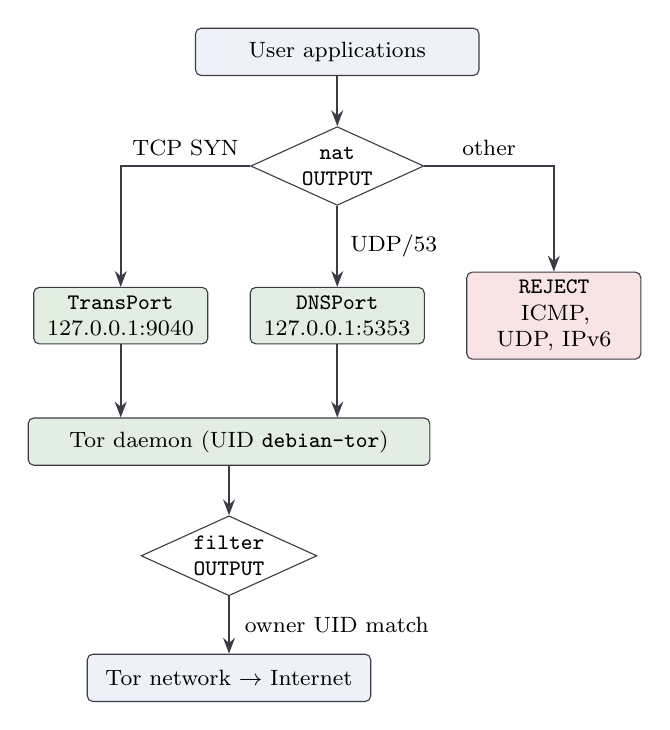
\begin{tikzpicture}
  % row 1
  \node[blk, minimum width=36mm] (app) at (0,0) {User applications};
  % row 2
  \node[dec] (nat) at (0,-1.45) {\texttt{nat}\\\texttt{OUTPUT}};
  % row 3: three outcomes
  \node[tor,  text width=20mm] (trans) at (-2.75,-3.35) {\texttt{TransPort}\\127.0.0.1:9040};
  \node[tor,  text width=20mm] (dns)   at ( 0.0,-3.35) {\texttt{DNSPort}\\127.0.0.1:5353};
  \node[drop, text width=20mm] (drop)  at ( 2.75,-3.35) {\texttt{REJECT}\\ICMP, UDP, IPv6};
  % row 4
  \node[tor, minimum width=51mm] (tor) at (-1.375,-4.95) {Tor daemon (UID \texttt{debian-tor})};
  % row 5
  \node[dec] (flt) at (-1.375,-6.4) {\texttt{filter}\\\texttt{OUTPUT}};
  % row 6
  \node[blk, minimum width=36mm] (net) at (-1.375,-7.95) {Tor network $\rightarrow$ Internet};

  \draw[flow] (app) -- (nat);
  % labels sit beside the lines, never on them
  \draw[flow] (nat.west) -| (trans.north)
        node[pos=0.25, above, font=\footnotesize] {TCP SYN};
  \draw[flow] (nat.south) -- (dns.north)
        node[midway, right=1pt, font=\footnotesize] {UDP/53};
  \draw[flow] (nat.east) -| (drop.north)
        node[pos=0.25, above, font=\footnotesize] {other};
  \draw[flow] (trans.south) -- (trans.south |- tor.north);
  \draw[flow] (dns.south)   -- (dns.south |- tor.north);
  \draw[flow] (tor) -- (flt);
  \draw[flow] (flt) -- (net)
        node[midway, right=2pt, font=\footnotesize] {owner UID match};
\end{tikzpicture}
\caption{Outbound packet path. All user traffic is either redirected into
Tor or rejected. Apart from DHCP on the local link, only the Tor
daemon's own connections may leave a physical interface.}
\label{fig:arch}
\end{figure}

\subsection{Tor Configuration}
The Tor client is configured with three listeners, all bound to
loopback, and the options listed in Table~\ref{tab:torrc}. Stream isolation flags on the
\texttt{TransPort} keep connections to different destinations on
separate circuits, which limits cross-site linkability.
\texttt{ClientUseIPv6 0} stops Tor itself from selecting IPv6 relays,
which would otherwise conflict with the disabled IPv6 stack.

\begin{table}[t]
\centering
\caption{Tor Client Configuration ({\normalfont\ttfamily /etc/tor/torrc})}
\label{tab:torrc}
\renewcommand{\arraystretch}{1.2}
\footnotesize
\begin{tabularx}{\columnwidth}{|P{3.6cm}|Y|}
\hline
\textbf{Option (value)} & \textbf{Purpose} \\ \hline
\texttt{SocksPort} (9050)            & SOCKS proxy for aware applications \\ \hline
\texttt{TransPort} (9040)            & Receives NAT-redirected TCP \\ \hline
\texttt{DNSPort} (5353)              & Resolves redirected DNS via Tor \\ \hline
\texttt{VirtualAddrNetworkIPv4}      & Virtual range \texttt{10.192.0.0/10} \\ \hline
\texttt{AutomapHostsOnResolve}       & Maps names, incl.\ \texttt{.onion} \\ \hline
\texttt{IsolateDestAddr/Port}        & Per-destination circuits \\ \hline
\texttt{ClientUseIPv6} (0)           & No IPv6 relay connections \\ \hline
\end{tabularx}
\end{table}

\subsection{Firewall Rule Set}
The routing script is written to fail closed. It first sets every
built-in chain in both the IPv4 and IPv6 tables to \texttt{DROP}, and
only then flushes and rebuilds the rules. The script runs with
\texttt{set -euo pipefail}, so a failure part-way through leaves the
host with no connectivity rather than partial enforcement.
Listing~\ref{lst:rules} gives the essential rules.

\begin{lstlisting}[style=shell, float=t, caption={Core netfilter rules (abridged)}, label={lst:rules}, captionpos=b]
TOR=$(id -u debian-tor)
iptables -P OUTPUT DROP; ip6tables -P OUTPUT DROP
# NAT: exempt Tor, redirect DNS and TCP
iptables -t nat -A OUTPUT -m owner --uid-owner $TOR \
         -j RETURN
iptables -t nat -A OUTPUT -p udp --dport 53 \
         -j REDIRECT --to-ports 5353
iptables -t nat -A OUTPUT -o lo -j RETURN
iptables -t nat -A OUTPUT -p tcp --syn \
         -j REDIRECT --to-ports 9040
# FILTER: kill-switch
iptables -A OUTPUT -m conntrack --ctstate INVALID -j DROP
iptables -A OUTPUT -m conntrack \
         --ctstate ESTABLISHED,RELATED -j ACCEPT
iptables -A OUTPUT -m owner --uid-owner $TOR \
         -p tcp --syn -j ACCEPT
iptables -A OUTPUT -o lo -j ACCEPT
iptables -A OUTPUT -p udp --sport 68 --dport 67 -j ACCEPT
iptables -A OUTPUT -j REJECT
\end{lstlisting}

Packets that connection tracking drops as \texttt{INVALID} deserve
attention. Without that rule, a TCP packet in an unexpected state could
miss the NAT \texttt{SYN} match and be emitted unproxied, which is a
known leak in naive transparent proxy configurations.

\subsection{Eliminating the Early-Boot Window}
A common flaw in transparent Tor setups is to order the firewall
\emph{after} \texttt{network.target}. DHCP, NTP and connectivity checks
can then run on the clearnet before the rules exist. Specter OS sets
\texttt{DefaultDependencies=no} on the routing unit and orders it with
\texttt{Before=network-pre.target}. Because this target is passive, the
unit also declares \texttt{Wants=network-pre.target}, which pulls it
into the boot transaction. The \texttt{systemd} manager guarantees that
the target
is reached before any network management service configures an
interface~\cite{systemd}. A \texttt{sysctl.d} drop-in, applied even
earlier by \texttt{systemd-sysctl}, disables IPv6 and ICMP echo
replies. The optional kernel parameter \texttt{ipv6.disable=1} removes
the IPv6 stack before user space starts at all. Figure~\ref{fig:boot}
shows the resulting ordering.

\begin{figure}[t]
\centering
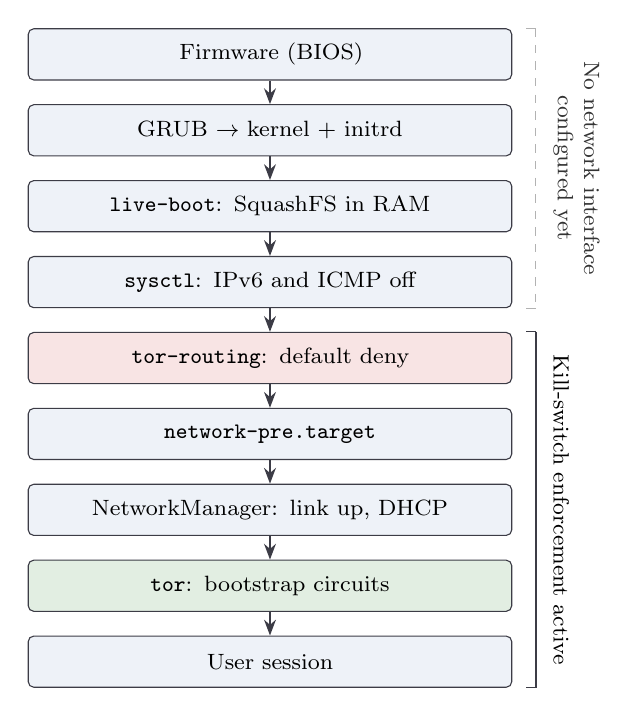
\begin{tikzpicture}[
    stage/.style={blk, text width=60mm, minimum height=6.5mm, inner sep=2pt},
    node distance=3mm]
  \node[stage]                  (fw)   {Firmware (BIOS)};
  \node[stage, below=of fw]     (grub) {GRUB $\rightarrow$ kernel + initrd};
  \node[stage, below=of grub]   (live) {\texttt{live-boot}: SquashFS in RAM};
  \node[stage, below=of live]   (sys)  {\texttt{sysctl}: IPv6 and ICMP off};
  \node[stage, below=of sys, fill=dropfill] (rt) {\textbf{\texttt{tor-routing}}: default deny};
  \node[stage, below=of rt]     (pre)  {\texttt{network-pre.target}};
  \node[stage, below=of pre]    (nm)   {NetworkManager: link up, DHCP};
  \node[stage, below=of nm, fill=torfill] (tor) {\texttt{tor}: bootstrap circuits};
  \node[stage, below=of tor]    (ui)   {User session};
  \foreach \a/\b in {fw/grub,grub/live,live/sys,sys/rt,rt/pre,pre/nm,nm/tor,tor/ui}
    \draw[flow] (\a) -- (\b);

  % enforcement bracket on the right of the stages it covers
  \coordinate (kt) at ($(rt.north east)+(3mm,0)$);
  \coordinate (kb) at ($(ui.south east)+(3mm,0)$);
  \draw[thick, draw=line] (kt) -- (kb);
  \draw[draw=line] (kt) -- ++(-1.2mm,0);
  \draw[draw=line] (kb) -- ++(-1.2mm,0);
  \node[font=\footnotesize, rotate=-90, anchor=south] at ($(kt)!0.5!(kb)+(1mm,0)$)
        {Kill-switch enforcement active};
  % pre-enforcement span
  \coordinate (pt) at ($(fw.north east)+(3mm,0)$);
  \coordinate (pb) at ($(sys.south east)+(3mm,0)$);
  \draw[draw=gray!60, dashed] (pt) -- (pb);
  \draw[draw=gray!60] (pt) -- ++(-1.2mm,0);
  \draw[draw=gray!60] (pb) -- ++(-1.2mm,0);
  \node[font=\footnotesize, text=gray!40!black, rotate=-90, anchor=south, align=center]
        at ($(pt)!0.5!(pb)+(1mm,0)$)
        {No network interface\\configured yet};
\end{tikzpicture}
\caption{Boot ordering. No interface is ever configured without
enforcement, because the kill-switch is installed before
\texttt{network-pre.target}.}
\label{fig:boot}
\end{figure}

\subsection{Live, Amnesic Operation}
The root filesystem is stored as an XZ-compressed SquashFS image.
\texttt{live-boot} locates it at boot and mounts it beneath a RAM-backed
overlay. All writes go to memory and are discarded at power-off, so no
browsing history, logs or Tor state survive between sessions unless
persistence is explicitly added (Section~\ref{sec:limits}).

% ------------------------------------------------------------------
\section{Implementation}
\label{sec:impl}

The system is assembled by hand rather than with the
\texttt{live-build} framework, so that each stage can be inspected.
Figure~\ref{fig:build} summarises the pipeline.

\begin{figure}[t]
\centering
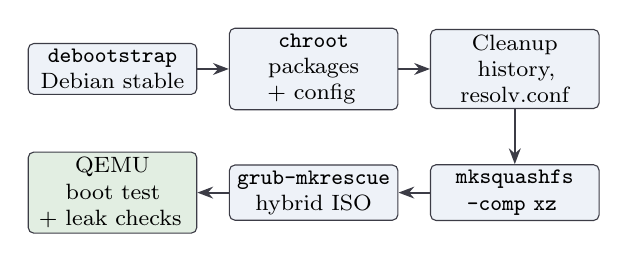
\begin{tikzpicture}[node distance=4mm and 4mm]
  \node[blk, text width=20mm, inner sep=2pt] (a) {\texttt{debootstrap}\\Debian stable};
  \node[blk, text width=20mm, inner sep=2pt, right=of a] (b) {\texttt{chroot}\\packages + config};
  \node[blk, text width=20mm, inner sep=2pt, right=of b] (c) {Cleanup\\history, \mbox{resolv.conf}};
  \node[blk, text width=20mm, inner sep=2pt, below=7mm of c] (d) {\texttt{mksquashfs}\\\texttt{-comp xz}};
  \node[blk, text width=20mm, inner sep=2pt, left=of d] (e) {\texttt{grub-mkrescue}\\hybrid ISO};
  \node[tor, text width=20mm, inner sep=2pt, left=of e] (f) {QEMU boot test\\+ leak checks};
  \draw[flow] (a) -- (b);
  \draw[flow] (b) -- (c);
  \draw[flow] (c) -- (d);
  \draw[flow] (d) -- (e);
  \draw[flow] (e) -- (f);
\end{tikzpicture}
\caption{Build pipeline from a minimal Debian base to a tested ISO.}
\label{fig:build}
\end{figure}

\subsection{Base System and Packages}
The base system is a minimal Debian stable tree created by
\texttt{debootstrap}. Inside a \texttt{chroot}, with the host's
\texttt{/dev}, \texttt{/proc}, \texttt{/sys} and \texttt{/run}
bind-mounted, the following packages are installed: \texttt{tor},
\texttt{iptables}, \texttt{network-manager}, \texttt{macchanger},
\texttt{live-boot}, \texttt{live-config} and the kernel
(\texttt{linux-image-amd64}), together with basic utilities. The Specter OS configuration
files are then copied to their target paths and the units are enabled.
Before the tree is compressed, the build host's \texttt{resolv.conf},
shell history and package caches are removed so that no build-host
information is embedded in the image.

\subsection{Compression and Bootloader}
XZ is chosen for SquashFS because it gives the best compression ratio
of the available algorithms, at the cost of build time
(Table~\ref{tab:comp}). An early prototype assembled the El Torito boot
image by hand with \texttt{grub-mkimage}. It produced an invalid boot
record and failed in QEMU with ``could not read from CDROM.'' Using
\texttt{grub-mkrescue}, which generates \texttt{boot.img},
\texttt{core.img}, the boot catalog and the module set consistently,
resolved the problem.

\begin{table}[t]
\centering
\caption{SquashFS Compression Trade-offs}
\label{tab:comp}
\renewcommand{\arraystretch}{1.2}
\footnotesize
\begin{tabularx}{\columnwidth}{|P{1.6cm}|Y|}
\hline
\textbf{Algorithm} & \textbf{Characteristics} \\ \hline
\texttt{xz}   & Highest ratio, smallest image, slowest build (selected) \\ \hline
\texttt{zstd} & Good ratio, fast decompression \\ \hline
\texttt{gzip} & Balanced, universally supported \\ \hline
\texttt{lz4}  & Fastest, lowest ratio \\ \hline
\end{tabularx}
\end{table}

\subsection{Development Issues}
Table~\ref{tab:errors} records the main issues met during development
and how each was resolved. They may be useful to others who build live
systems by hand.

\begin{table}[t]
\centering
\caption{Issues Encountered During Development}
\label{tab:errors}
\renewcommand{\arraystretch}{1.2}
\footnotesize
\begin{tabularx}{\columnwidth}{|P{2.6cm}|Y|}
\hline
\textbf{Symptom} & \textbf{Cause and resolution} \\ \hline
No DNS in chroot & Missing \texttt{resolv.conf}; copy from host, delete before packaging \\ \hline
{\ttfamily unable to allocate pty} & \texttt{sudo} used while already root in chroot; run directly \\ \hline
ISO not bootable & Hand-built El Torito image; rebuilt with \texttt{grub-mkrescue} \\ \hline
Locale warnings & Locale not generated; set \texttt{en\_US.UTF-8} \\ \hline
Unit fails to parse & Malformed section header; corrected to \texttt{[Unit]} \\ \hline
\end{tabularx}
\end{table}

\begin{table*}[!t]
\centering
\caption{Leak Verification Tests: Expected and Observed Results}
\label{tab:tests}
\renewcommand{\arraystretch}{1.2}
\footnotesize
\begin{tabularx}{\textwidth}{|P{3.5cm}|P{3.7cm}|Y|Y|}
\hline
\textbf{Test} & \textbf{Expected (hardened)} & \textbf{Observed: hardened image} & \textbf{Observed: initial image} \\ \hline
Tor check API (\texttt{curl}) & \texttt{"IsTor":true} & Not reached (Tor stalled at 45\,\%) & Not reached (same stall) \\ \hline
\texttt{dig} to external resolver & Answered by Tor DNSPort & No answer; 0 UDP/53 frames & No answer; 0 UDP/53 frames \\ \hline
\texttt{ping} external host & Fails (rejected) & 0/3 replies; 0 ICMP frames & \textbf{3/3 replies; 5 ICMP frames} \\ \hline
UDP probe (NTP, port 123) & Rejected & 0 frames & 0 frames (UDP rule) \\ \hline
IPv6 traffic & None (no IPv6 stack) & \texttt{disable\_ipv6=1}; 0 frames & \textbf{14 IPv6 frames} \\ \hline
Stop \texttt{tor.service}, retry & No connectivity at all & No connectivity; 0 frames & \textbf{Ping 2/2 replies; 4 frames} \\ \hline
Boot order (\texttt{systemd}) & Routing precedes network & Routing 1.5\,s before NM & \textbf{NM 0.6--0.9\,s before routing} \\ \hline
NIC capture (\texttt{filter-dump}) & DHCP, ARP and Tor TCP only & DHCP, ARP and Tor TCP only & \textbf{Also ICMP and IPv6} \\ \hline
\multicolumn{4}{|l|}{NM = NetworkManager. Boot-order values cover two boots per image.} \\ \hline
\end{tabularx}
\end{table*}
% ------------------------------------------------------------------
\section{Verification Methodology and Results}
\label{sec:eval}

Each leak vector in Table~\ref{tab:vectors} is paired with a test that
can be run inside the booted system (Table~\ref{tab:tests}).

\subsection{Test Setup}
Two images were built from the same Debian~13 base (kernel 6.12,
Tor 0.4.9.15, \texttt{iptables} 1.8.11 with the \texttt{nf\_tables}
backend): an \emph{initial} image using the routing script, unit file
and \texttt{torrc} of the project's first commit, and a \emph{hardened}
image using the files described in Section~\ref{sec:design}. Each image
was booted under QEMU 11.1 with KVM, 1\,GB of RAM and user-mode
networking. QEMU's \texttt{filter-dump} object recorded every frame the
virtual NIC emitted from power-on to power-off, which gives an
observation point outside the guest. A self-test unit, added to the test
images only, ran the probes of Table~\ref{tab:tests} after boot,
printed the results to the serial console and powered the guest off.

\subsection{Results}
Table~\ref{tab:tests} summarises the observations. The hardened image
emitted no ICMP, DNS, other UDP or IPv6 frames, and no frame at all
after Tor was stopped. Its routing unit completed 1.5\,s before
NetworkManager started, in both boots. The initial image leaked ICMP
and IPv6, kept answering pings after Tor was stopped, and started
NetworkManager 0.6--0.9\,s \emph{before} its firewall rules were in
place. \texttt{systemd-analyze verify} also showed why: the malformed
section header in the initial unit caused its \texttt{After=} ordering
to be ignored.

Tor did not complete bootstrapping in either image within the
self-test window. Its log reported repeated
\texttt{CONNECTRESET} and \texttt{CONNECTREFUSED} errors from relays and
stalled at 45\,\%. Because the initial image applies no TCP filtering
and failed in the same way, we attribute this to the test network
rather than to the rule set. The counters of the hardened rule set
confirm this: every one of Tor's 194 new connections was accepted, and
the final \texttt{REJECT} rule matched only the 4 probe packets.
The \texttt{IsTor} check, Tor DNS and Tor latency could therefore not
be measured here.

% ------------------------------------------------------------------
\section{Discussion and Limitations}
\label{sec:limits}

\textbf{Application layer.} A transparent proxy on its own does not make
applications anonymous: a redirected browser still sends its own fingerprintable headers, fonts
and canvas data. Specter OS protects the network layer. Application
privacy requires Tor Browser~\cite{torbrowser}.

\textbf{Single-host enforcement.} Unlike Whonix, a compromised
application running as root can rewrite the firewall. Gateway
isolation through virtualisation is stronger but costs portability.

\textbf{UDP.} Tor carries only TCP streams, so non-DNS UDP services
(VoIP, QUIC, online games) are unavailable by design.

\textbf{Hardware identifiers.} MAC addresses are visible to the local
network. Randomisation with \texttt{macchanger} at boot is planned but
not yet enforced.

\textbf{Restrictive networks.} Where the network resets Tor connections,
as in our tests, the fail-closed design leaves the user offline; Tor
bridges would address this.

\textbf{Evaluation scope.} The results come from two virtual-machine
boots per image and are not yet repeated on physical hardware.

\textbf{Not audited.} The system has not undergone independent security
review and should be treated as a research platform.

% ------------------------------------------------------------------
\section{Future Work}
\label{sec:future}
Planned extensions include LUKS-encrypted persistence, a UEFI
and Secure Boot path, automatic MAC randomisation before
\texttt{network-pre.target}, AppArmor confinement of user applications,
migration of the rule set to \texttt{nftables}, and reproducible builds
so that third parties can verify that a published ISO matches its
source.

% ------------------------------------------------------------------
\section*{Code Availability Statement}
The source code, build scripts and configuration files of Specter OS
(Version~1.0, November 2026) are available at
\url{https://github.com/HAMZOO0/Specter-OS}.

% ------------------------------------------------------------------
{\footnotesize
\begin{thebibliography}{10}
\raggedright
\setlength{\itemsep}{1pt}

\bibitem{dingledine2004tor}
R.~Dingledine, N.~Mathewson, and P.~Syverson, ``Tor: The
second-generation onion router,'' in \emph{Proc. 13th USENIX Security
Symp.}, San Diego, CA, USA, 2004, pp.~303--320.

\bibitem{torproject2024transparent}
The Tor Project, ``TransparentProxy,'' Tor Project Community Wiki.
[Online]. Available:
\url{https://gitlab.torproject.org/legacy/trac/-/wikis/doc/TransparentProxy}.
Accessed: Nov.~22, 2026.

\bibitem{tails}
Tails Developers, ``Tails: The amnesic incognito live system.''
[Online]. Available: \url{https://tails.net}. Accessed: Nov.~22, 2026.

\bibitem{whonix}
Whonix Developers, ``Whonix: Superior internet privacy.''
[Online]. Available: \url{https://www.whonix.org}. Accessed: Nov.~22, 2026.

\bibitem{qubes}
J.~Rutkowska and R.~Wojtczuk, ``Qubes OS architecture,'' Invisible
Things Lab, Tech. Rep., 2010.

\bibitem{murdoch2005low}
S.~J. Murdoch and G.~Danezis, ``Low-cost traffic analysis of Tor,'' in
\emph{Proc. IEEE Symp. Security and Privacy}, 2005, pp.~183--195.

\bibitem{webrtcleak}
N.~Al-Fannah, ``One leak will sink a ship: WebRTC IP address leaks,''
in \emph{Proc. Int. Carnahan Conf. Security Technology (ICCST)}, 2017.

\bibitem{systemd}
systemd Project, ``systemd.special(7): \texttt{network-pre.target},''
freedesktop.org manual pages. [Online]. Available:
\url{https://www.freedesktop.org/software/systemd/man/systemd.special.html}.
Accessed: Nov.~22, 2026.

\bibitem{torbrowser}
M.~Perry, E.~Clark, S.~Murdoch, and G.~Koppen, ``The design and
implementation of the Tor Browser,'' The Tor Project, Tech. Rep.
[Online]. Available:
\url{https://2019.www.torproject.org/projects/torbrowser/design/}.
Accessed: Nov.~22, 2026.

\end{thebibliography}
}

\end{document}
